\section{Introducci\'on y objetivos}
Hacia fines del siglo XIX y principios del siglo XX (\alert{revisar}), con el prop'osito de estudiar la estructura interna de una pieza musical, 
Heinrich Schenker elabor'o una teor'ia de la coherencia tonal en la m'usica conocido como \texttt{an'alisis schenkeriano}.
En su teor'ia, Schenker postula que la superficie musical (lo que se escucha) es resultado de sucesivas transformaciones que sufre una estructura b'asica fundamental 
denominada por el autor la \emph{ursatz}\footnote{estructura fundamental en alem'an}. Estas transformaci'ones estan descriptas en t'erminos de reglas de reescritura que permiten 
a partir de una cierta ursatz llegar a una pieza musical competa. Dado que la ursatz es la estructura fundamental, 'esta s'olo contiene las notas que dan la impronta de la pieza, 
que luego son elaboradas usando las reglas de reescritura.

Si bien el an'alisis schenkeriano fue concebido para llevar la ursatz a una pieza musical completa, queda claro que se lo puede utilizar tambi'en para estimar
cual podr'ia ser la ursatz de un cierta superficie musical. De esta forma, al utilizar la teor'ia ``en sentido contrario'', en vez de hablar en t'erminos de elaboraci'ones de 
la ursatz a la superficie musical, habr'ia que hacerlo en terminos de reducciones. Definida como lo opuesto a una elaboraci'on, una reducci'on permite especificar que una cierta 
nota dentro de un grupo es la estructuralmente mas importante, y que todo el resto es una \texttt{elaboraci'on} de esta. 
Dado que esta relaci'on de reducci'on/elaboraci'on se puede aplicar recursivamente, naturalmente emerge una relaci'on 
jer'arquica entre las notas de una pieza musical.  En esta jerarqu'ia, el nivel m'as bajo es lo que se encuentra escrito en la partitura, y a medida que se sube de nivel se 
encuentran diferentes versiones de la misma pieza musical cada vez menos elaboradas. En la figura \ref{fig_analisis_schenkeriano} se exhibe un ejemplo de dicho an'alisis.


\begin{figure}[h]
\begin{center}
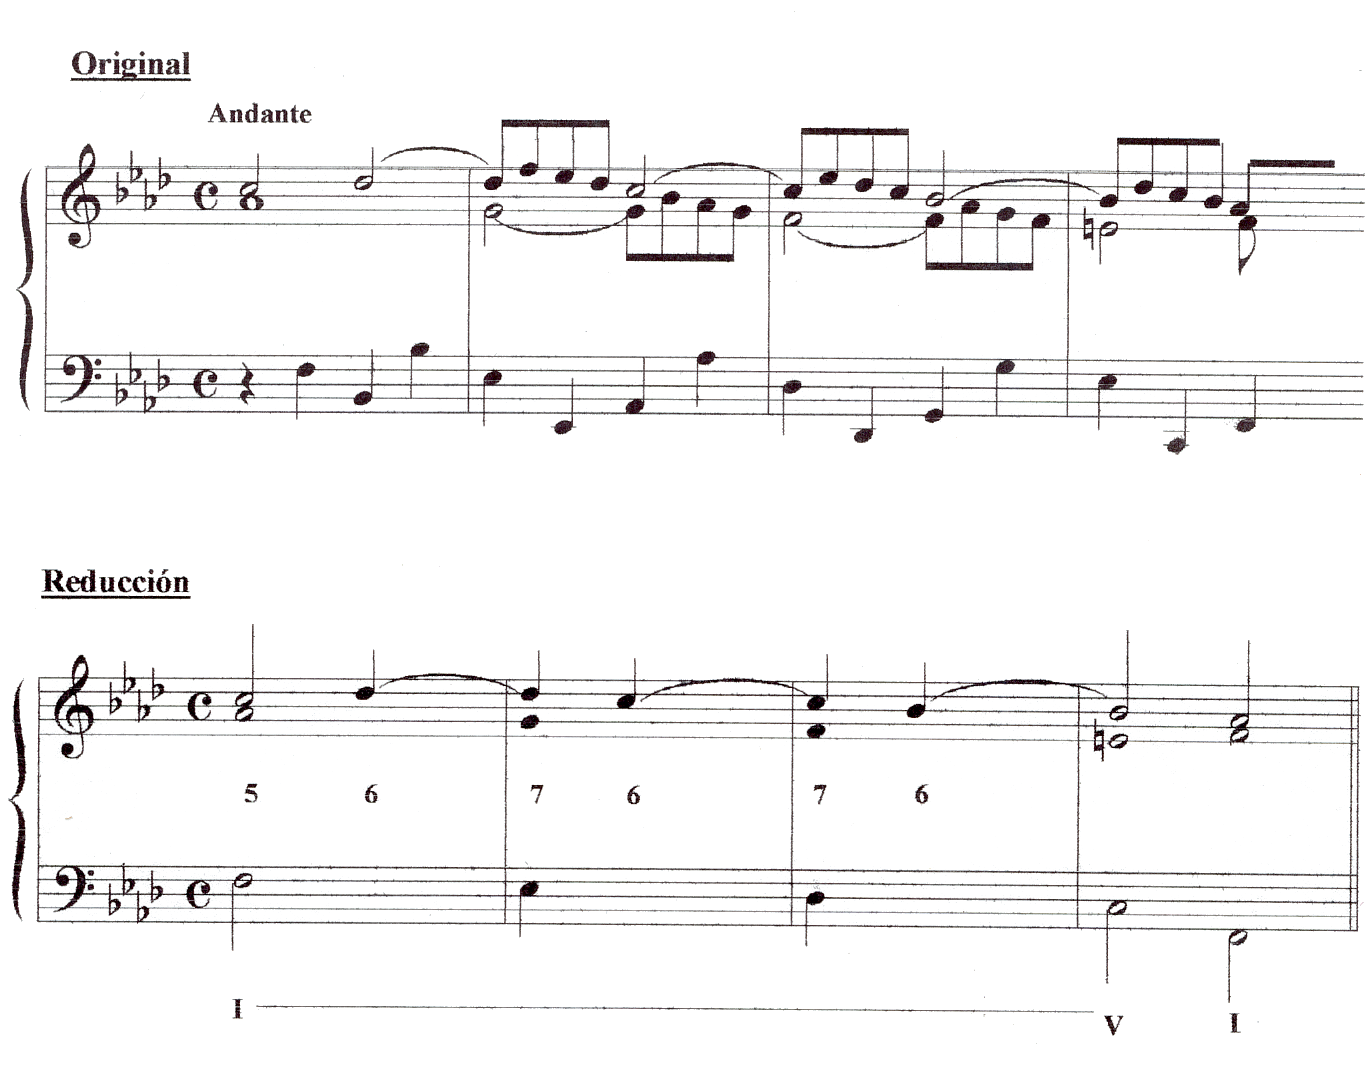
\includegraphics[width=12cm]{images/schenkerian_example}
\label{fig_analisis_schenkeriano}
\newline \alert{poner una imagen mas copada}
\end{center}
\end{figure}

En esta figura, los sucesivos pentagramas muestran relaciones de reducci'on, as'i simplificando el tema con el objeto de llevarlo a una representaci'on m'as abstracta.

El parecido de este tipo de relaciones con las relaci'ones utilizadas por Noam Chomsky para analizar el lenguaje natural es notable. 
Si bien en la teor'ia de Chomsky las relaciones son relaciones del tipo ``es un'', y en la teor'ia de Schenker son del tipo ``es una elaboraci'on de'', 
estas se enmarcan matem'aticamente en el mismo lugar.  

En 1983, el m'usico Fred Lerdahl y el ling\"uista Ray Jackendoff publicaron el libro 
\texttt{A Generative Theory of Tonal Music}(GTTM) donde proponen una gram'atica para analizar la m'usica t'erminos parecidos a los de Schenker. 
Lo interesante de este trabajo es el fundamento que se le da a la elecci'on de las reglas de la gram'atica, puesto que proponen una teor'ia que tomando los conceptos claves
de la teor'ia schenkeriana se basa en supuestos cognitivos de naturaleza computacional.

El objetivo del trabajo de Lerdahl y Jackendoff es principalmente tener modelizar el proceso mediante el cual se estructura la percepci'on de la m'usica. 
Este modelo consiste en una serie de reglas de preferencia. Cada regla tiene asociado un predicado booleano $P$, un valor de preferencia $v$ y una acci'on interpretativa 
$I$, de modo que si el predicado $P$ es verdadero, entonces aportan $v$ unidades a la preferencia a interpretar de acuerdo a $I$ cierto fen'omeno. 
Para ejemplificar, a continuaci'on se cita una regla de preferencia de los autores. Esta regla es una de las reglas asociadas a lo que los autores 
llaman agrupamiento, que b'asicamente consiste en agrupar notas que tienen significancia de frase\footnote{M'as adelante se explicar'a esto con mayor detalle}.
\newline

\begin{center}
\texttt{GPR 1} Evite fuertemente grupos que contengan solamente un evento.
\end{center}

En este caso, el predicado booleano es aquel que es verdadero solamente con grupos de cardinalidad uno, y el valor de preferencia es fuertemente negativo a la acci'on interpretativa
de decidir que el grupo en cuesti'on debe contener 'unicamente al evento que contiene. 

Si bien un modelo de este tipo es generativo en el sentido de que podr'ia ser utilizado por una computadora tanto para analizar una pieza musical como para 
\texttt{generar} una nueva, es importante notar que este no es su objetivo. 
Puede verse claramente como la regla \emph{GPR 1} si bien es suficientemente rigurosa como para luego poder corroborarla emp'iricamente, no lo es como para construir un 
programa que haga un an'alisis utilizando esta regla: es necesario determinar el valor de preferencia y aprender las relaci'ones entre los distintos valores de preferencia para luego 
tomar una desici'on.  

De esta forma se discrimina entre \texttt{modelos generativos}, que son aquellos que eventualmente podr'ian utilizarse para generar aquello que explican, y 
\texttt{modelos de 'indole generativo} que fueron hechos con el objeto de generar aquello que explican.  El hecho de que sea necesario definir expl'icitamente los valores de preferencias
sumado a que este modelo no es de 'indole generativo plantea el interrogante de si realmente este enfoque es el adecuado para para modelar la cognici'on musical con aprendizaje 
autom'atico. 

De este modo, el objetivo de este trabajo es utilizar el conocimiento generado por trabajos como el de Lerdahl y Jackendoff como medio para establecer propiedades que un modelo de 
'indole generativo deber'ia cumplir. Teniendo estas propiedades, luego es posible construir un modelo desvinculado de la idea de gram'atica, que respete 
ciertos criterios fundamentales. Si se logra conseguir un modelo de estas caracter'isticas se podr'an validar emp'iricamente los criterios en base a los que el modelo fue construido 
(y por lo tanto las teor'ias cognitivas que motivaron los criterios) a trav'es de analizar las piezas musicales generadas por el modelo.

Para poder avanzar en pos del objetivo recien planteado, es necesario primero sentar un vocabulario para luego poder contextualizarlo. De esta forma, las siguientes dos
secci'ones hablaran sobre background. Luego se har'a un breve resumen sobre el estado del arte en este tema, para luego abordar el trabajo en concreto de esta tesis.

